\begin{figure}[hbtp]
\centering
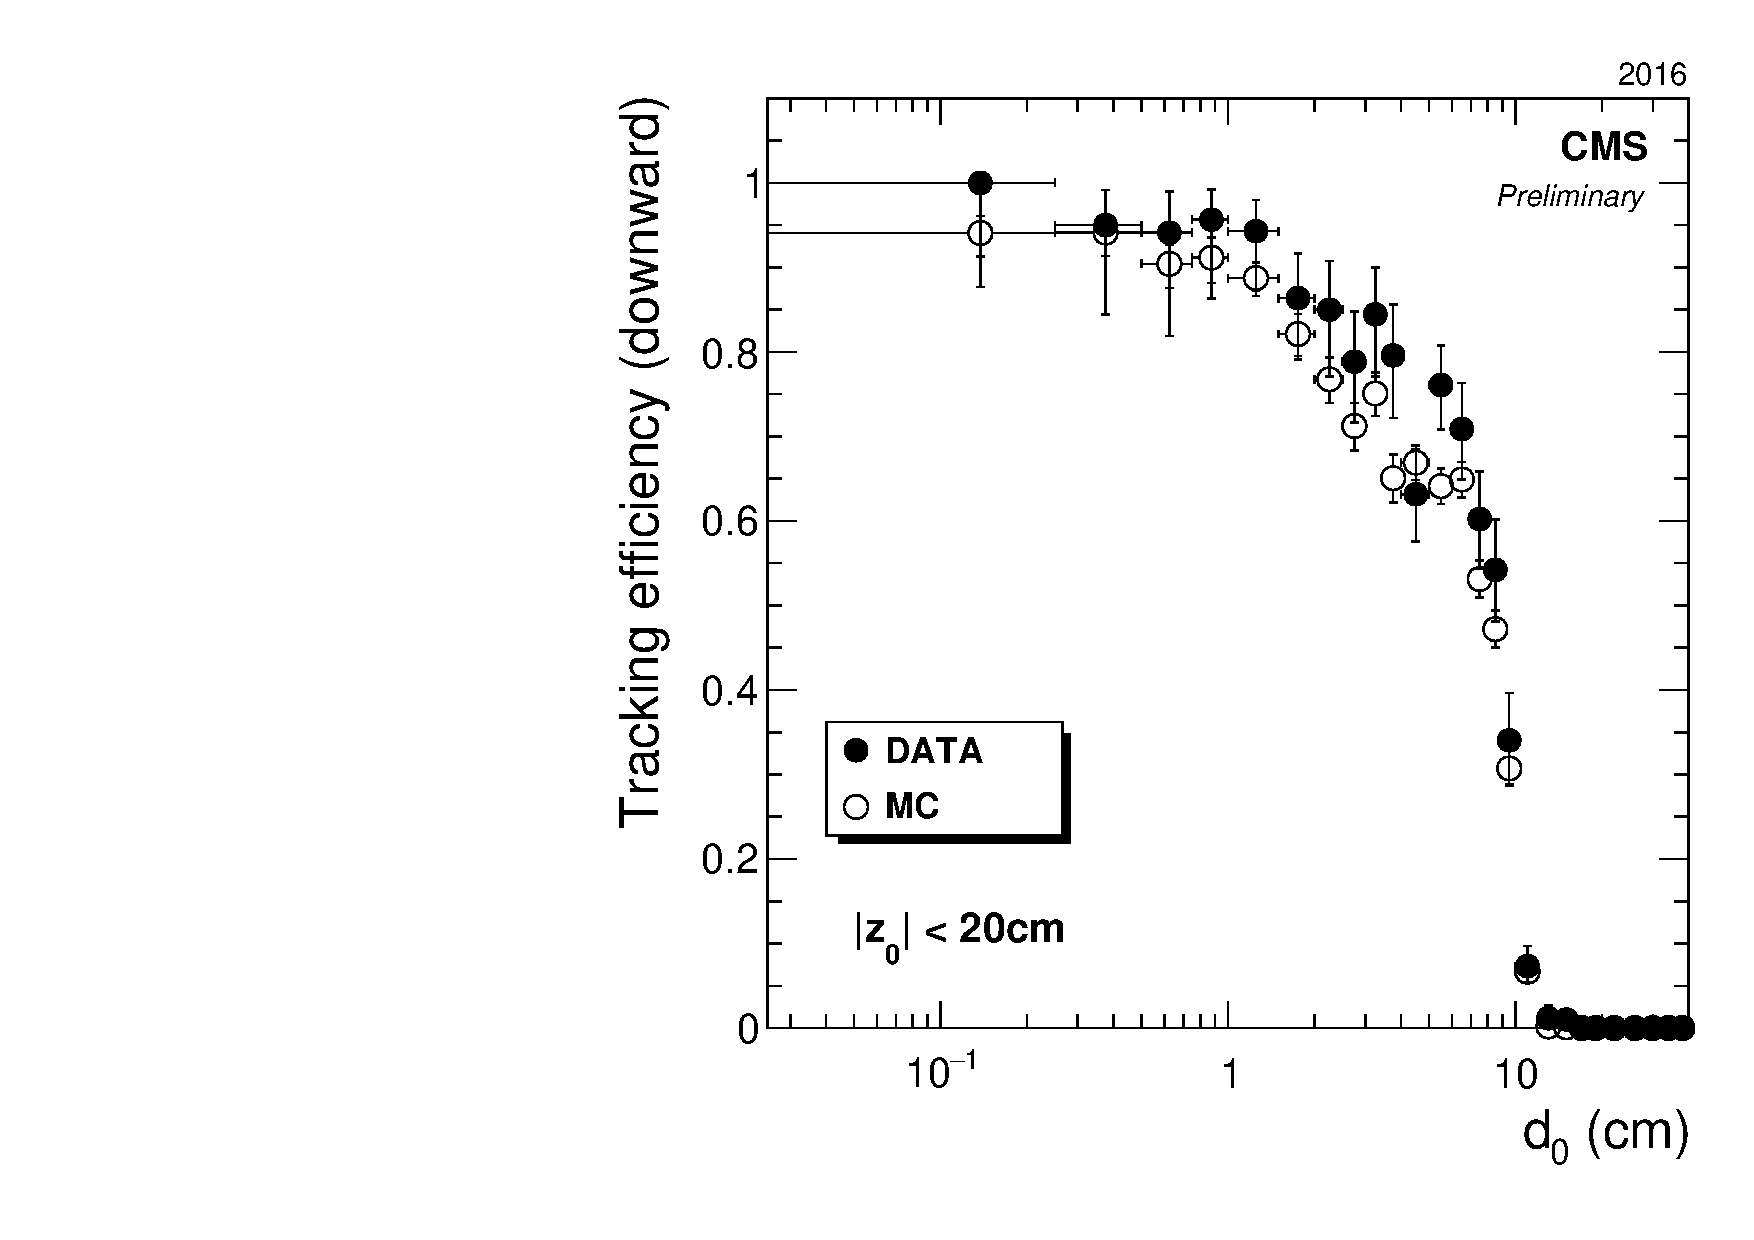
\includegraphics[width=0.4\textwidth]{figures/tracking_eff/2016/Eff0vsD0.pdf}
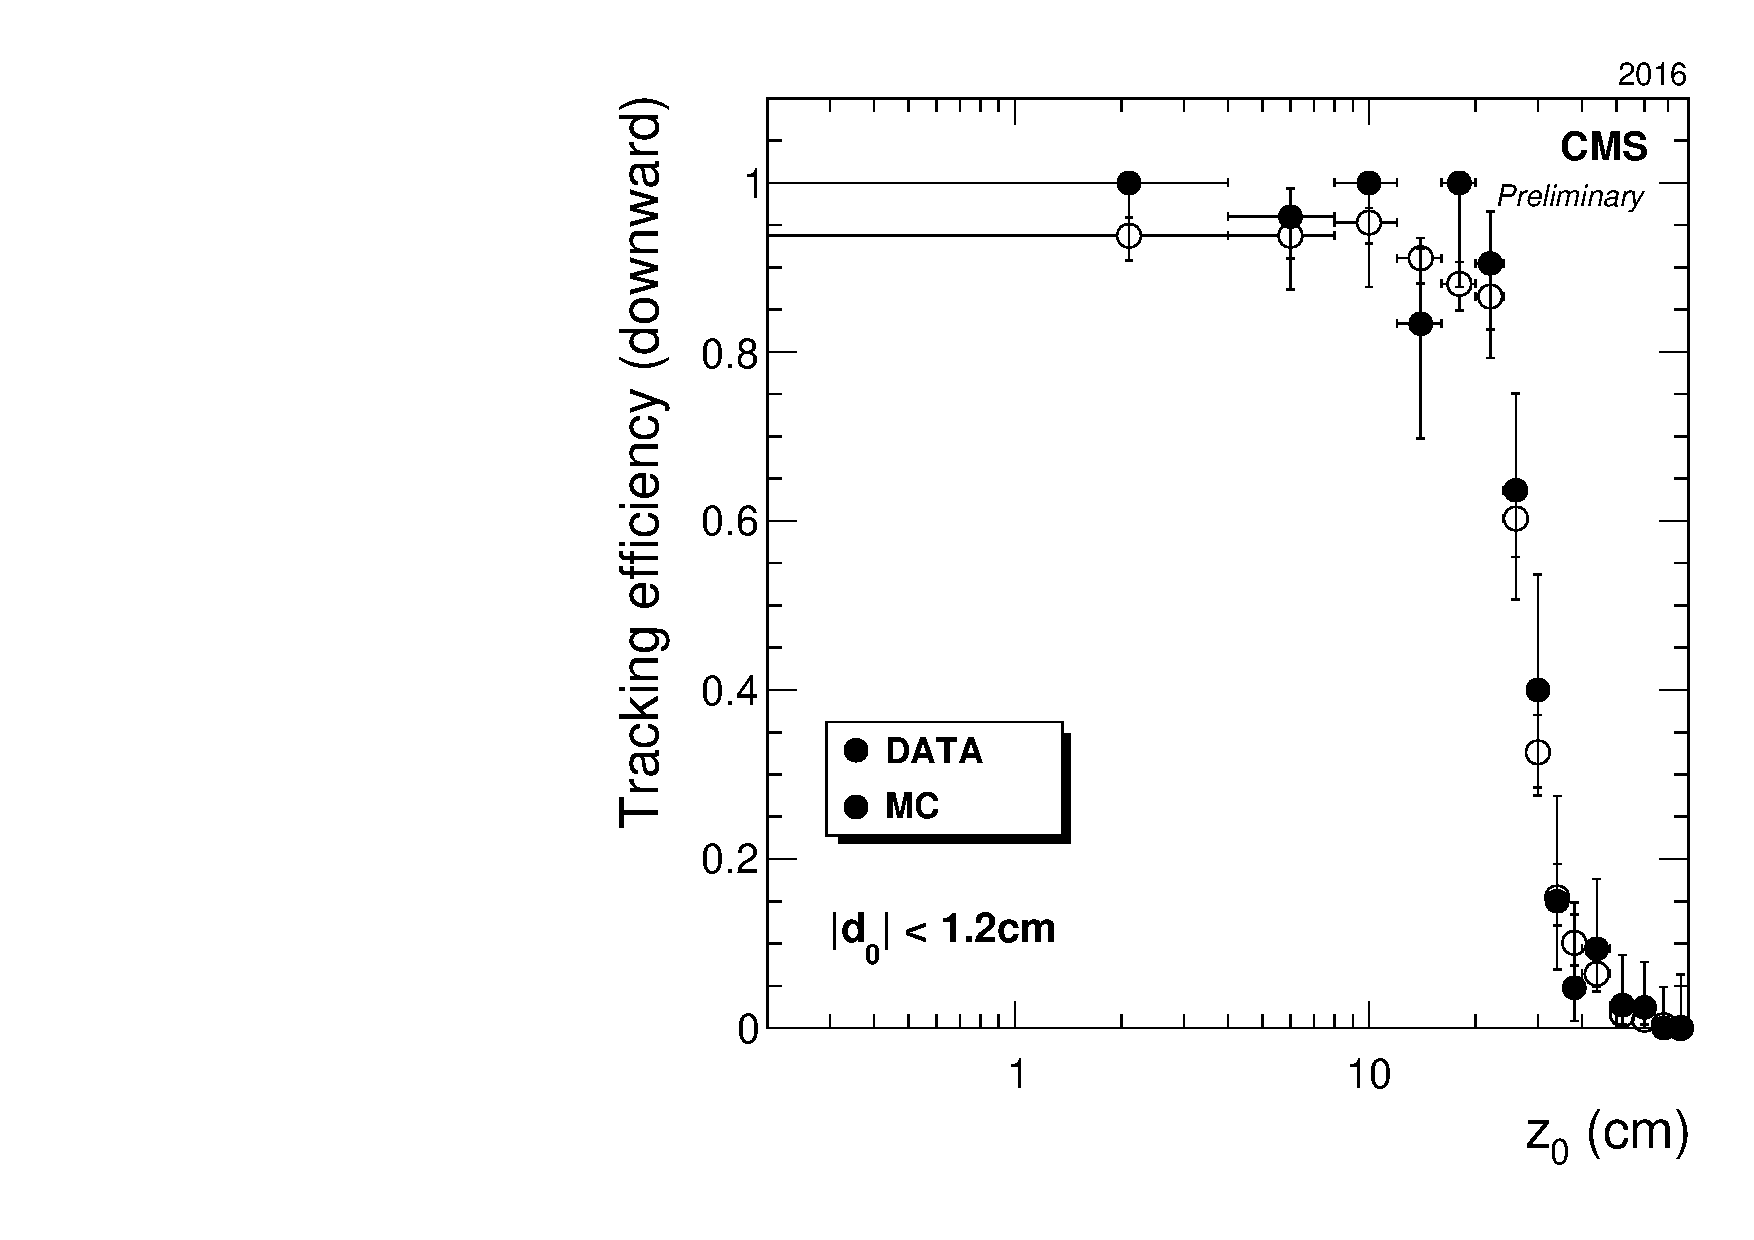
\includegraphics[width=0.4\textwidth]{figures/tracking_eff/2016/Eff0vsZ0.pdf}
\\
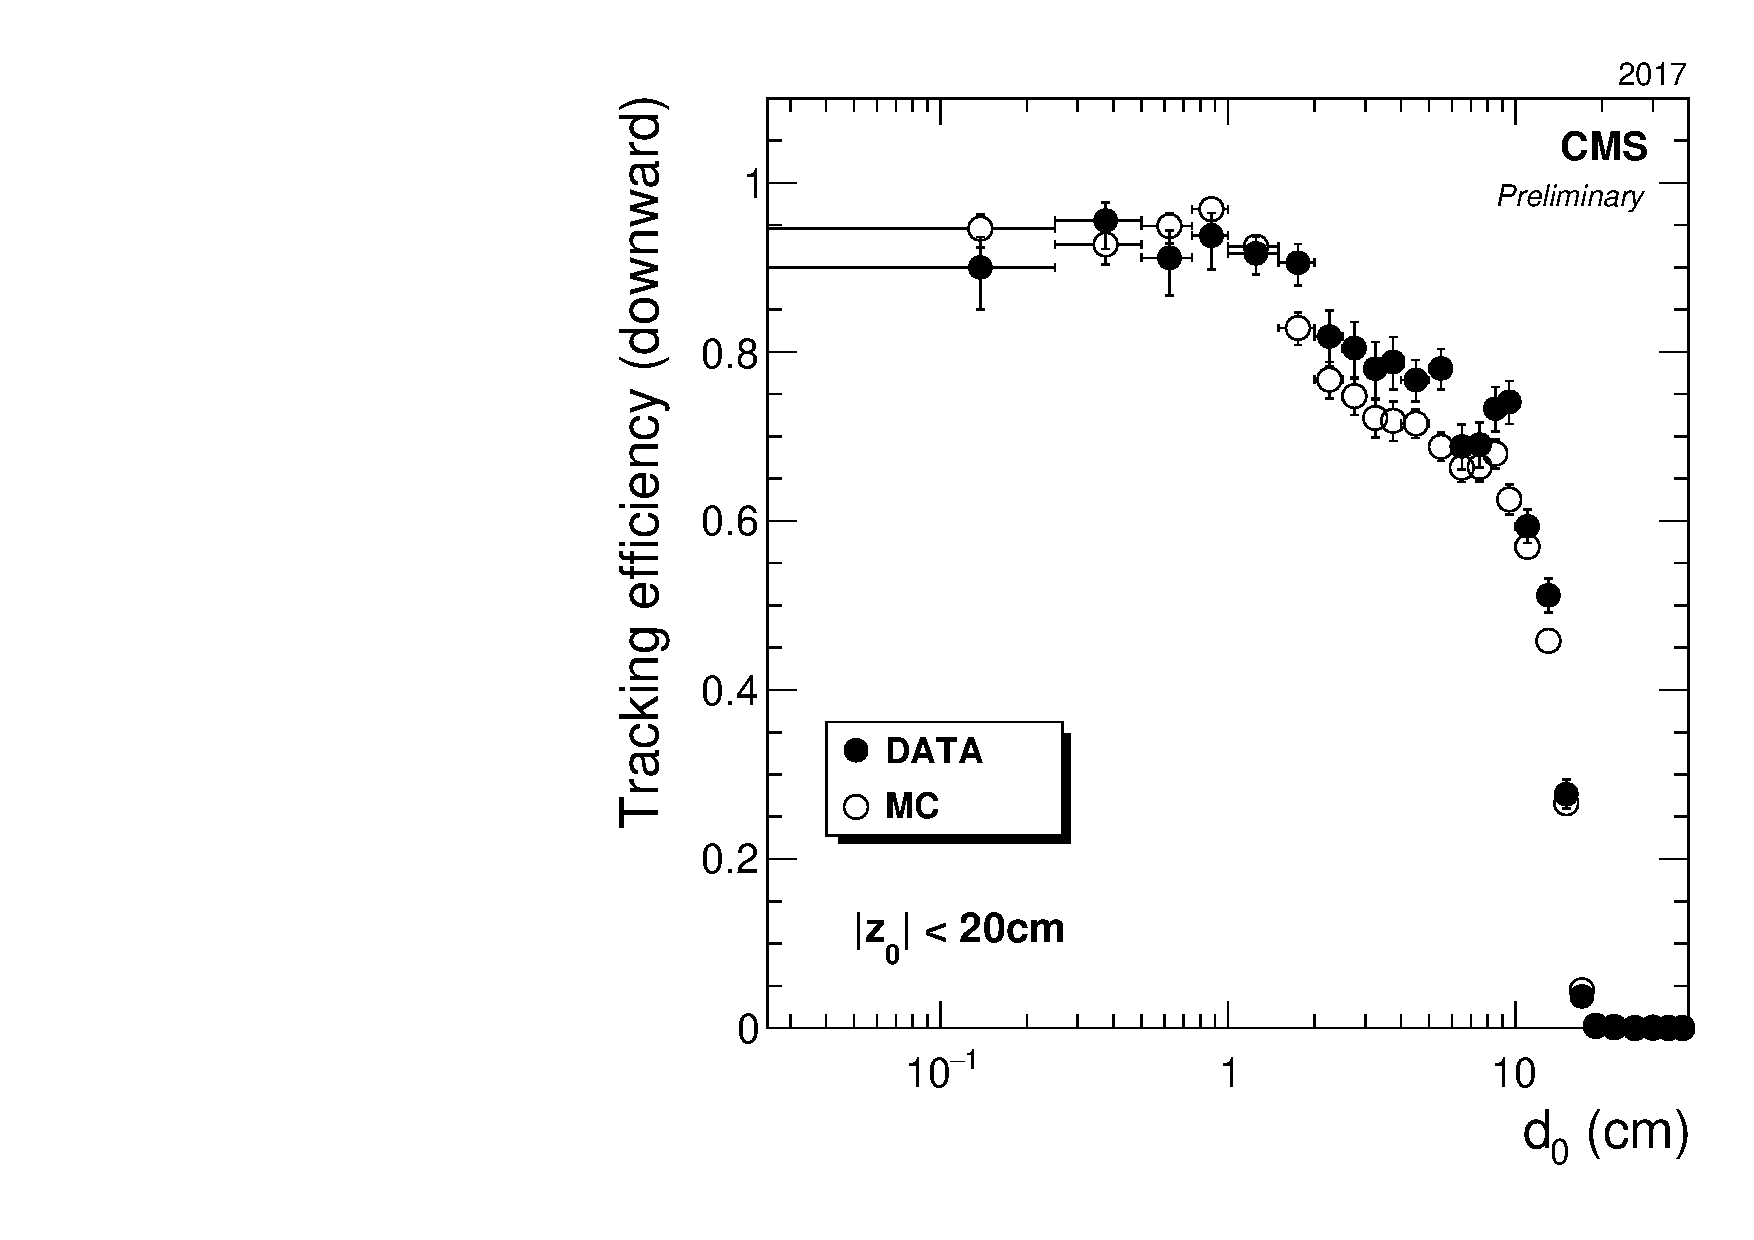
\includegraphics[width=0.4\textwidth]{figures/tracking_eff/2017/Eff0vsD0.pdf}
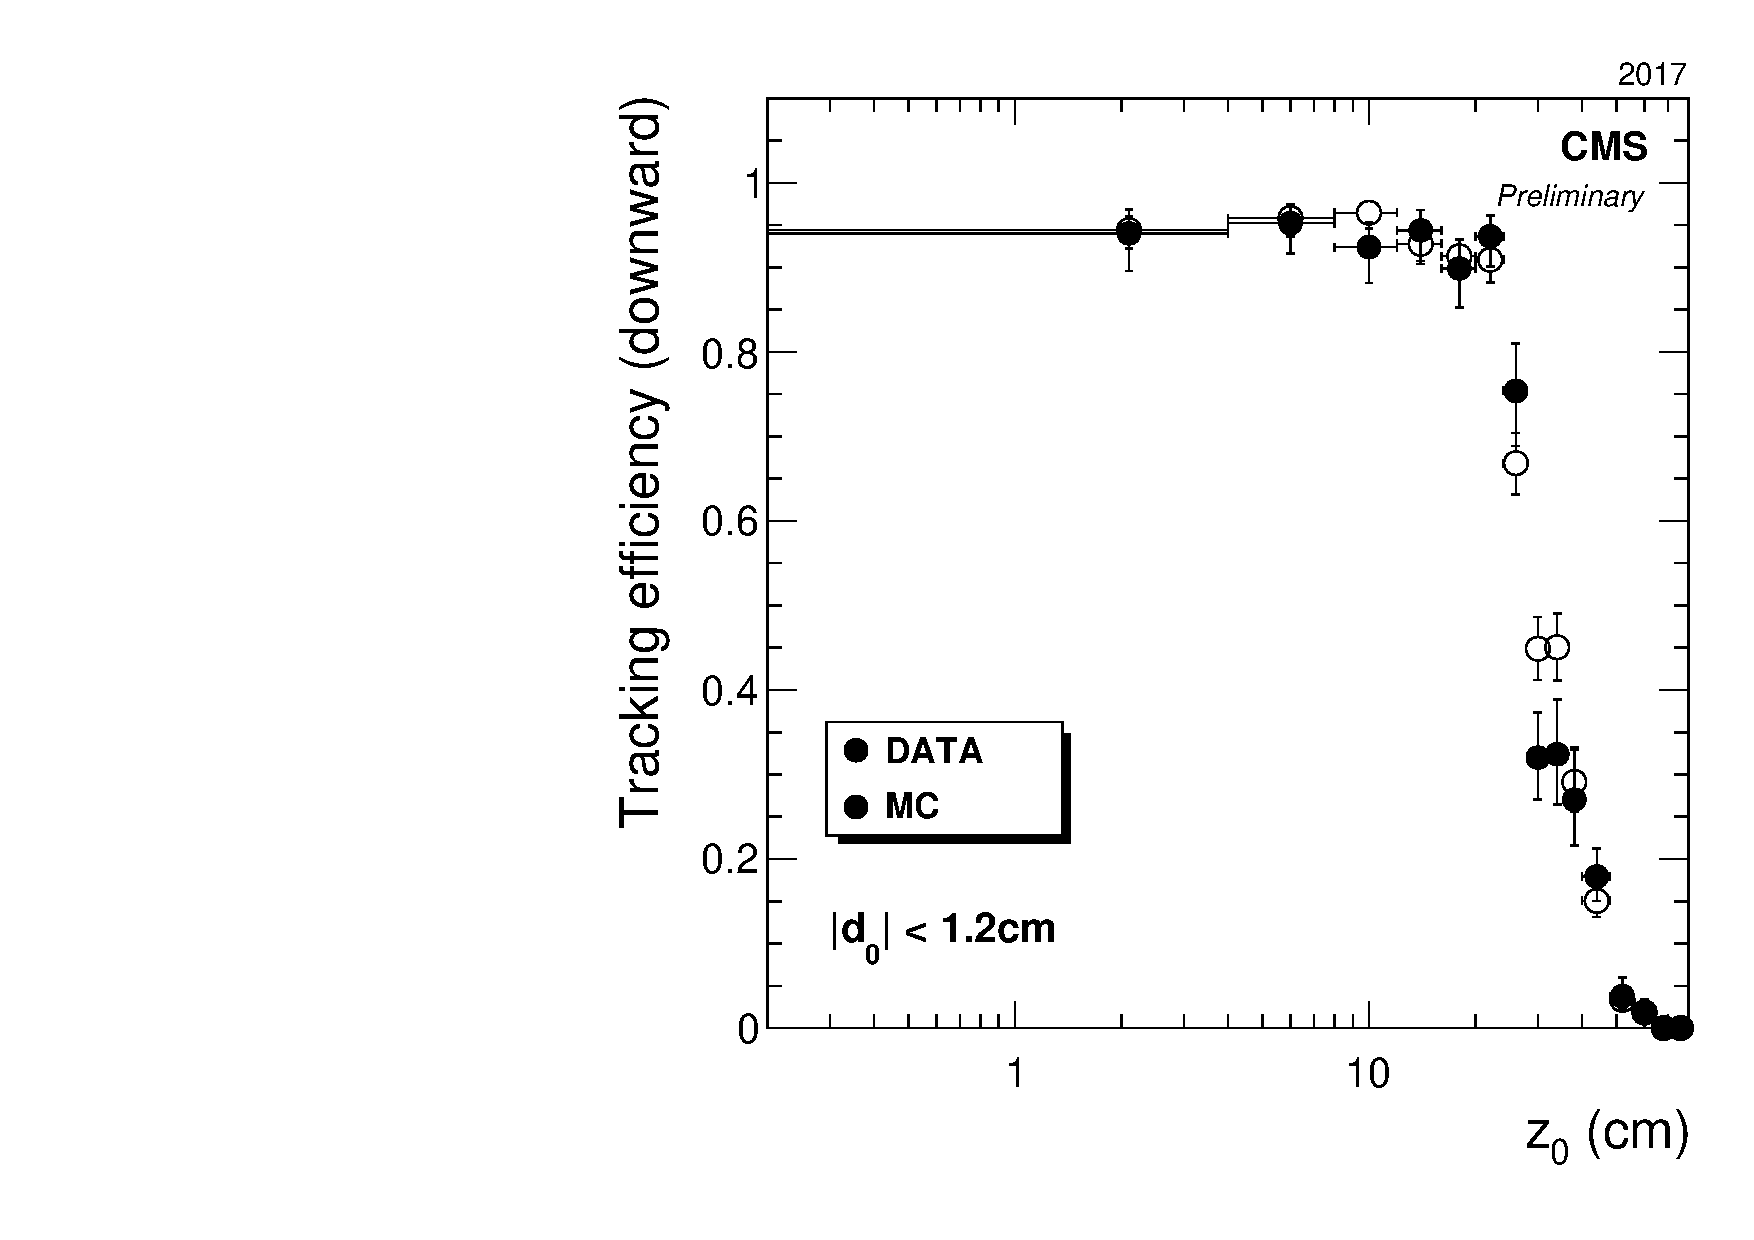
\includegraphics[width=0.4\textwidth]{figures/tracking_eff/2017/Eff0vsZ0.pdf}
\\
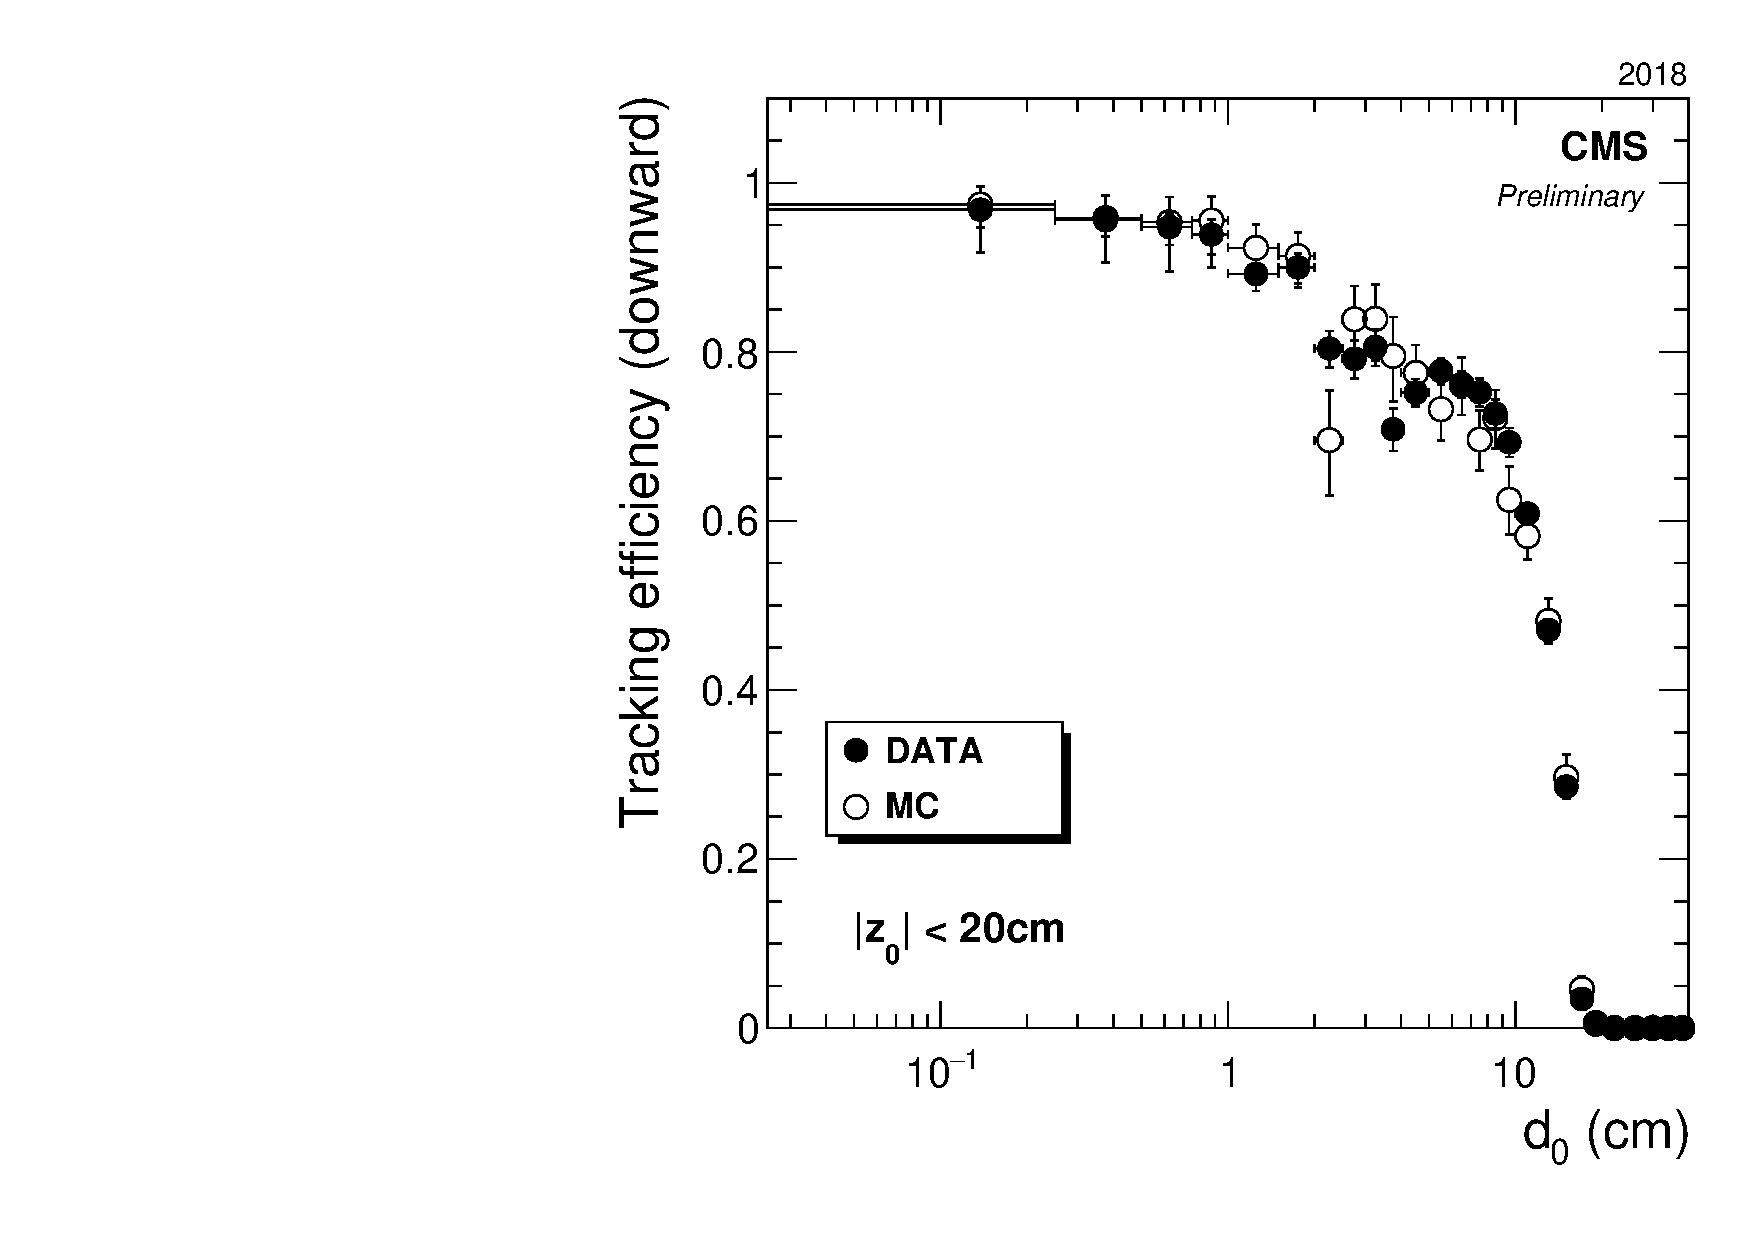
\includegraphics[width=0.4\textwidth]{figures/tracking_eff/2018/Eff0vsD0.pdf}
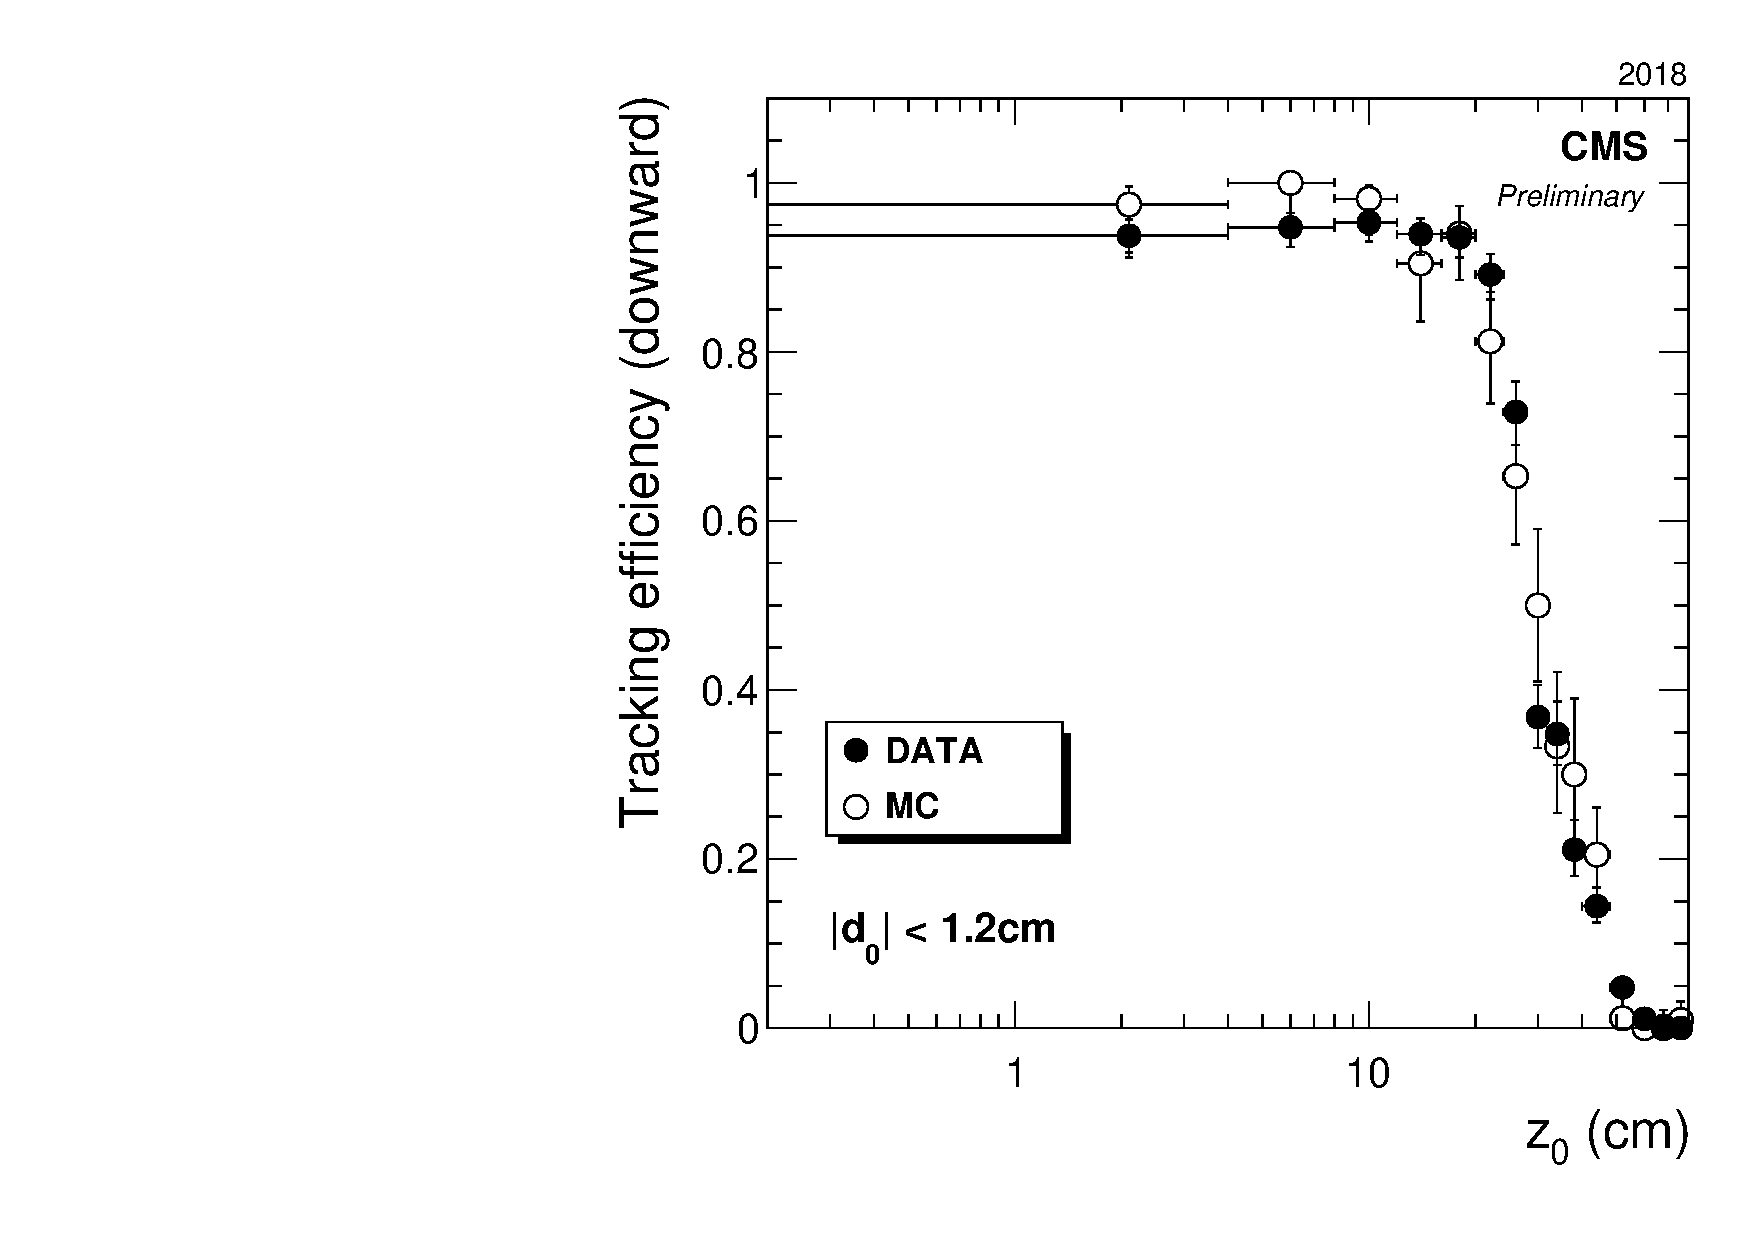
\includegraphics[width=0.4\textwidth]{figures/tracking_eff/2018/Eff0vsZ0.pdf}
\caption{Measured downward tracking efficiency in 2016 (top), 2017 (middle), and 2018 (bottom) versus transverse impact parameter (left) and longitudinal impact parameter (right) in data and simulation. The longitudinal (transverse) impact parameter is constrained to less than \SI{20}{\cm} (\SI{1.2}{\cm}) when plotting against the transverse (longitudinal) impact parameter.}
\label{displaced_trk_eff_vs_d0dz}
\end{figure}